%%%%%%%%%%%%%%%%%%%%%%%%%%%%%%%%%%%%%%%%%
% Beamer Presentation
% LaTeX Template
% Version 1.0 (10/11/12)
%
% This template has been downloaded from:
% http://www.LaTeXTemplates.com
%
% License:
% CC BY-NC-SA 3.0 (http://creativecommons.org/licenses/by-nc-sa/3.0/)
%
%%%%%%%%%%%%%%%%%%%%%%%%%%%%%%%%%%%%%%%%%

%-------------------------------------------------------------------------------
%	PACKAGES AND THEMES
%-------------------------------------------------------------------------------

\documentclass{beamer}
\usepackage{xcolor}
\usepackage{graphicx}
\usepackage{tikz}
\usepackage{listings}
\usepackage{multicol}
\usepackage[autoload=false]{jlcode}

\DeclareMathOperator{\diag}{diag}

\definecolor{applegreen}{rgb}{0.55, 0.71, 0.0}
\definecolor{blue(ncs)}{rgb}{0.0, 0.45, 0.60}
\definecolor{burgundy}{rgb}{0.5, 0.0, 0.13}

\definecolor{cadet}{rgb}{0.33, 0.41, 0.47}
\definecolor{airforceblue}{rgb}{0.36, 0.54, 0.66}

\mode<presentation> {

\usetheme{CambridgeUS}

\usecolortheme{wolverine}

\definecolor{gold}{HTML}{D4A017}
\definecolor{darkgold}{HTML}{B7950B}

\setbeamercolor{palette primary}{bg=cadet,fg=white}
\setbeamercolor{palette secondary}{bg=airforceblue,fg=white}
\setbeamercolor{palette tertiary}{bg=black,fg=white}
\setbeamercolor{palette quaternary}{bg=cadet,fg=white}

\setbeamercolor{frametitle}{bg=airforceblue,fg=white}

\setbeamercolor{section number projected}{bg=black,fg=cadet}
\setbeamercolor{item}{fg=black,bg=cadet}

\setbeamertemplate{page number in head/foot}[framenumber]
}

\usepackage{graphicx} % Allows including images
\usepackage{booktabs} % Allows the use of \toprule, \midrule and \bottomrule in tables

%-------------------------------------------------------------------------------
%	TITLE PAGE
%-------------------------------------------------------------------------------

\title[BDDC Preconditioned P-Multigrid]{BDDC Preconditioned P-Multigrid for High-Order Finite Elements} % The short title appears at the bottom of every slide, the full title is only on the title page

\author{Jeremy L Thompson} % Your name
\institute[CU Boulder] % Your institution as it will appear on the bottom of every slide, may be shorthand to save space
{University of Colorado, Boulder \\ % Your institution for the title page
\medskip
\textit{jeremy@jeremylt.org} % Your email address
}
\date{April 4, 2022} % Date, can be changed to a custom date

\begin{document}

\begin{frame}
\titlepage % Print the title page as the first slide
\end{frame}

%-------------------------------------------------------------------------------

\begin{frame}
\begin{center}
\frametitle{Funding}

This work is supported by the Department of Energy, National Nuclear Security Administration, Predictive Science Academic Alliance Program (PSAAP) under Award Number DE-NA0003962.

\end{center}
\end{frame}
 
%-------------------------------------------------------------------------------

\begin{frame}
\frametitle{Overview} % Table of contents slide, comment this block out to remove it
\tableofcontents % Throughout your presentation, if you choose to use \section{} and \subsection{} commands, these will automatically be printed on this slide as an overview of your presentation
\end{frame}

%-------------------------------------------------------------------------------
%	PRESENTATION SLIDES
%-------------------------------------------------------------------------------

%-------------------------------------------------------------------------------
\section{Introduction}
%-------------------------------------------------------------------------------

\begin{frame}
\begin{center}
\frametitle{Big Picture}

\begin{itemize}

\item High-order matrix-free representations of PDEs are better suited to modern hardware than sparse matrices\\

~\\

\item High-order matrix-free representations require preconditioned\\iterative solvers\\

~\\

\item Local Fourier Analysis (LFA) provides sharp convergence estimates\\for these preconditioners\\

~\\

\item We investigate LFA of Balancing Domain Decomposition by Constraints (BDDC) for high-order element subdomains\\

~\\

\item We investigate LFA of $p$-multigrid with a BDDC smoother

\end{itemize}

\end{center}
\end{frame}

%-------------------------------------------------------------------------------
\section{High-Order Matrix-Free FEM}
%-------------------------------------------------------------------------------

\begin{frame}
\begin{center}
\frametitle{Modern Hardware}

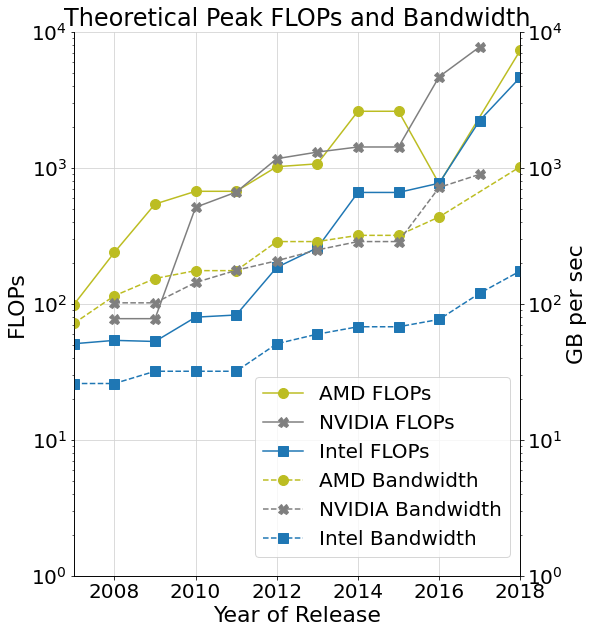
\includegraphics[height=5.5cm]{peakFlopsAndBandwidth_tall}
\hspace{1cm}
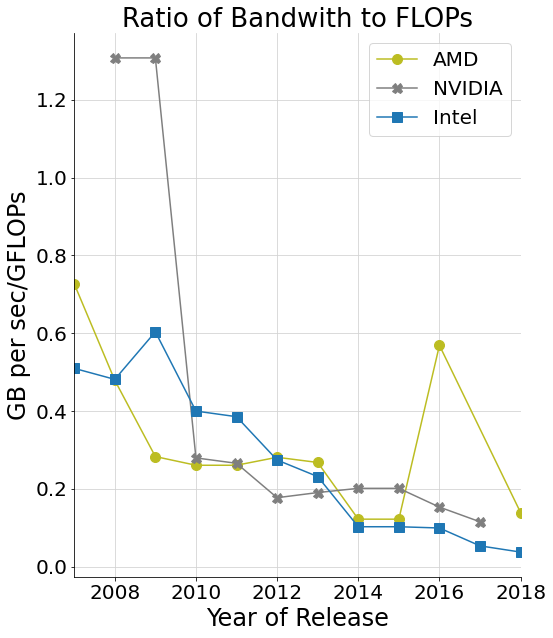
\includegraphics[height=5.5cm]{peakRatio_tall}

Modern hardware has lower memory bandwidth than FLOPs\\
(https://github.com/karlrupp/cpu-gpu-mic-comparison)

\end{center}
\end{frame}

%-------------------------------------------------------------------------------

\begin{frame}
\begin{center}
\frametitle{Benefits of Matrix-Free}

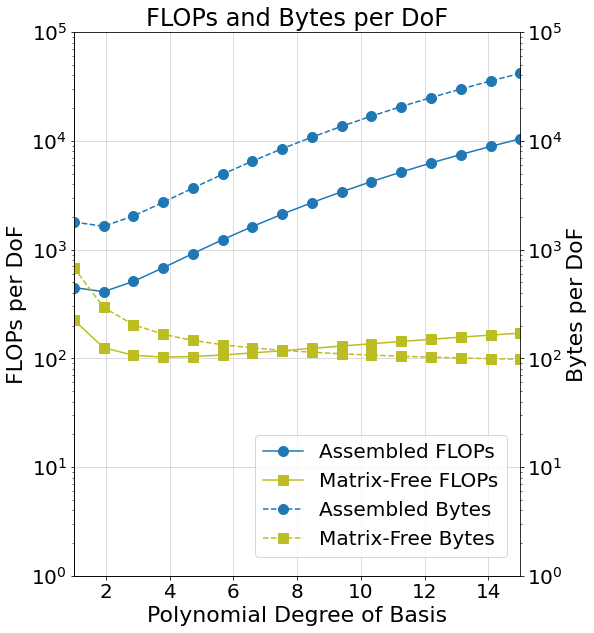
\includegraphics[height=5.5cm]{assembledVsMatrixFree_tall}
\hspace{1cm}
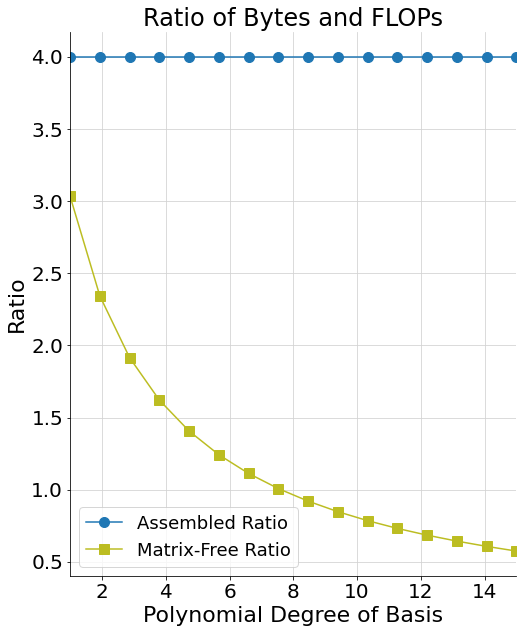
\includegraphics[height=5.5cm]{assembledVsMatrixFreeBalance_tall}

{\small Requirements for matrix-vector product with sparse matrix vs matrix-free\\ for screened Poisson $\nabla^2 u - \alpha^2 u = f$ in 3D}\\

For more details - see Rezgar Shakeri's talk Thursday, 13:05 in Session 10B

\end{center}
\end{frame}

%-------------------------------------------------------------------------------

\begin{frame}
\begin{center}
\frametitle{Matrix-Free Representation}

Weak form for an arbitrary second order PDE:\\

\begin{equation}
\begin{array}{c}
\text{find } u \in V \text{ such that for all } v \in V\\
\langle v, u \rangle = \int_{\Omega} v \cdot f_0 \left( u, \nabla u \right) + \nabla v : f_1 \left( u, \nabla u \right) = 0
\end{array}
\label{eq:weak_form}
\end{equation}

\begin{flushleft}
where
\end{flushleft}

\begin{itemize}

\item $\cdot$ - contraction over fields\\

\item $:$ - contraction over fields and spatial dimensions\\

\end{itemize}

~\\

Note: pointwise functions $f_0$ and $f_1$ don't depend upon the discretization\\

\end{center}
\end{frame}

%-------------------------------------------------------------------------------

\begin{frame}
\begin{center}
\frametitle{Matrix-Free Representation}

Galerkin form for an arbitrary second order PDE:\\

\begin{equation}
\sum_e \mathcal{E}^T \left[ \left( {\color{blue(ncs)}\mathbf{B}}_I^e \right)^T {\color{applegreen}\mathbf{W}}^e \Lambda \left( {\color{applegreen}f_0} \left( u^e, \nabla u^e \right) \right) + \sum_{i = 0}^{d - 1} \left( {\color{blue(ncs)}\mathbf{B}}_{\xi, i}^e \right)^T {\color{applegreen}\mathbf{W}}^e \Lambda \left( {\color{applegreen}f_1} \left( u^e, \nabla u^e \right) \right) \right] = 0
\label{eq:galerkin_form}
\end{equation}

\begin{itemize}

\item $\mathcal{E}$ - element assembly/restriction operator\\

\item ${\color{blue(ncs)}\mathbf{B}}_I^e$ - interpolation to quadrature points\\

\item ${\color{blue(ncs)}\mathbf{B}}_{\xi, i}^e$ - derivatives at quadrature points\\

\item ${\color{applegreen}\mathbf{W}}^e$ - quadrature weights\\

\item $\Lambda$ - pointwise multiplication at quadrature points\\

\item $u^e = {\color{blue(ncs)}\mathbf{B}}_I^e \mathcal{E}^e u$ and $\nabla u^e = \lbrace {\color{blue(ncs)}\mathbf{B}}_{\xi, i}^e \mathcal{E}^e u \rbrace_{i = 0}^{d - 1}$

\end{itemize}

\end{center}
\end{frame}

%-------------------------------------------------------------------------------

\begin{frame}
\begin{center}
\frametitle{libCEED Representation}

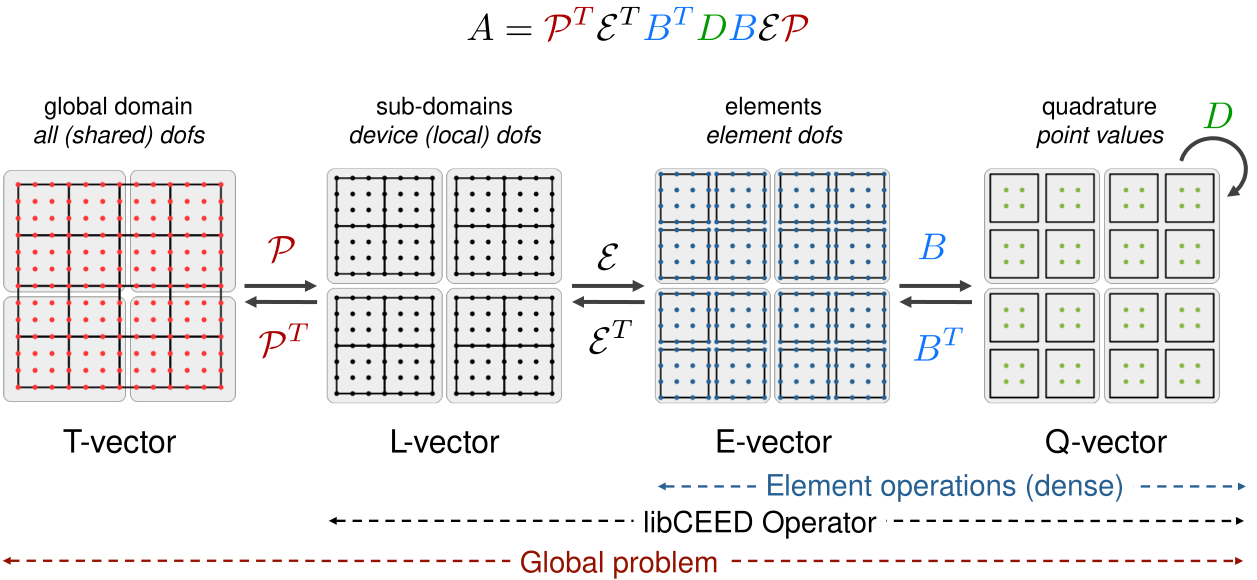
\includegraphics[height=4.5cm]{libCEEDAPI}

\begin{itemize}

\item ${\color{burgundy}\mathcal{P}}$ - parallel element assembly operator

\item $\mathcal{E}$ - local element assembly operator\\

\item ${\color{blue(ncs)}\mathbf{B}}$ - basis action operator\\

\item ${\color{applegreen}\mathbf{D}}$ - weak form and geometry at quadrature points\\

\end{itemize}

\end{center}
\end{frame}

%-------------------------------------------------------------------------------

\begin{frame}
\begin{center}
\frametitle{Preconditioning Required}

\begin{itemize}

\item Matrix-free representations require iterative solvers\\

~\\

\item Iterative solvers are sensitive to conditioning of the operator\\(among other factors)\\

~\\

\item High-order operators are ill-conditioned\\

~\\

\item Preconditioners are required for good convergence\\

~\\

\item LFA helps us tune these preconditioners\\

\end{itemize}

\end{center}
\end{frame}

%-------------------------------------------------------------------------------
\section{LFA of High-Order FEM}
%-------------------------------------------------------------------------------

\begin{frame}
\begin{center}
\frametitle{LFA Background}

Consider a scalar Toeplitz operator $L_h$ on the infinite 1D grid $G_h$

\begin{equation}
\begin{gathered}
L_h \mathrel{\hat{=}} \left[ s_\kappa \right]_h \left( \kappa \in V \right)\\
L_h w_h \left( x \right) = \sum_{\kappa \in V} s_\kappa w_h \left( x + \kappa h \right)
\end{gathered}
\end{equation}

\begin{flushleft}
where
\end{flushleft}

\begin{itemize}

\item $V \subset \mathbb{Z}$ is an index set

\item $s_\kappa \in \mathbb{R}$ are constant coefficients

\item $w_h \left( x \right)$ is an $l^2$ function on $G_h$

\end{itemize}

\end{center}
\end{frame}

%-------------------------------------------------------------------------------

\begin{frame}
\begin{center}
\frametitle{LFA Background}

Our function can be diagonalized by the standard Fourier modes:

~\\

~\\

If for all grid functions $\varphi \left( \theta, x \right)$

\vspace{-4mm}

\begin{equation}
L_h \varphi \left( \theta, x \right) = \tilde{L}_h \left( \theta \right) \varphi \left( \theta, x \right)
\end{equation}

then $\tilde{L}_h \left( \theta \right) = \sum_{\kappa \in V} s_\kappa e^{\imath \theta \kappa}$ is the {\bf symbol} of $L_h$\\

\end{center}
\end{frame}

%-------------------------------------------------------------------------------

\begin{frame}
\begin{center}
\frametitle{LFA Background}

For a $q \times q$ system of equations, the matrix symbol is given by:

\begin{equation}
\mathbf{L}_h =
\begin{bmatrix}
    L_h^{1, 1} && \cdots && L_h^{1, q}        \\
    \vdots               && \vdots && \vdots  \\
    L_h^{q, 1} && \cdots && L_h^{q, q}        \\
\end{bmatrix}
\hspace{0.5cm}
\Rightarrow
\hspace{0.5cm}
\tilde{\mathbf{L}}_h =
\begin{bmatrix}
    \tilde{L}_h^{1, 1} && \cdots && \tilde{L}_h^{1, q}  \\
    \vdots             && \vdots && \vdots              \\
    \tilde{L}_h^{q, 1} && \cdots && \tilde{L}_h^{q, q}  \\
\end{bmatrix}
\end{equation}

\end{center}
\end{frame}

%-------------------------------------------------------------------------------

\begin{frame}
\begin{center}
\frametitle{LFA of High-Order FEM}

For a scalar PDE operator on a single 1D finite element

\begin{equation}
\tilde{{\color{burgundy}\mathbf{A}}} \left( \theta \right) = \mathbf{Q}^T \left( {\color{burgundy}\mathbf{A}}^e \odot \left[ e^{\imath \left( x_j - x_i \right) \theta / h} \right] \right) \mathbf{Q}
\label{eq:symbolhighorder1d}
\end{equation}

\begin{flushleft}
where
\end{flushleft}

\begin{equation}
{\color{burgundy}\mathbf{A}}^e = {\color{blue(ncs)}\mathbf{B}}^T {\color{applegreen}\mathbf{D}} {\color{blue(ncs)}\mathbf{B}},
\hspace{5mm}
\mathbf{Q} =
\begin{bmatrix}
    \mathbf{I}   \\
    \mathbf{e}_0 \\
\end{bmatrix} =
\begin{bmatrix}
    1      && 0      && \cdots && 0      \\
    0      && 1      && \cdots && 0      \\
    \vdots && \vdots && \vdots && \vdots \\
    0      && 0      && \cdots && 1      \\
    1      && 0      && \cdots && 0      \\
\end{bmatrix}
\end{equation}

\end{center}
\end{frame}

%-------------------------------------------------------------------------------

\begin{frame}
\begin{center}
\frametitle{LFA of High-Order FEM}

Natural extension to multiple components and higher dimensions:\\

~\\

\begin{equation}
\tilde{{\color{burgundy}\mathbf{A}}} \left( \boldsymbol{\theta} \right) = \mathbf{Q}^T \left( {\color{burgundy}\mathbf{A}}^e \odot \left[ e^{\imath \left( \mathbf{x}_j - \mathbf{x}_i \right) \cdot \boldsymbol{\theta} / \mathbf{h}} \right] \right) \mathbf{Q}
\label{eq:symbolhighorder}
\end{equation}

~\\

\begin{columns}[onlytextwidth]
  \begin{column}{0.45\textwidth}
    \begin{center}
    Multiple Components:
    \end{center}
    \begin{equation}
    \mathbf{Q}_n = \mathbf{I}_n \otimes \mathbf{Q}
    \end{equation}
  \end{column}

  \begin{column}{0.45\textwidth}
    \begin{center}
    Multiple Dimensions:
    \end{center}
    \begin{equation}
    \mathbf{Q}_{nd} = \mathbf{Q} \otimes \mathbf{Q} \otimes \dots \otimes \mathbf{Q}
    \end{equation}
  \end{column}
\end{columns}

\end{center}
\end{frame}

%-------------------------------------------------------------------------------

\begin{frame}[fragile]
\begin{center}
\frametitle{Example: Scalar Poisson}

\begin{equation}
  \int \nabla v \nabla u = \int f v
\end{equation}

\begin{itemize}

\item ${\color{blue(ncs)}\mathbf{B}}$ - given by tensor $H^1$ Lagrange basis\\

\item ${\color{applegreen}\mathbf{D}}$ - given by quadrature weights and product\\

\end{itemize}

{\small
\begin{jllisting}[language=julia, style=jlcodestyle]
# mesh
dim = 1
mesh = Mesh1D(1.0)

# basis
p = 3
ncomp = 1
basis = TensorH1LagrangeBasis(p+1, p+1, ncomp, dim)

# weak form
function diffusionweakform(du::Array{Float64}, w::Array{Float64})
    return dv = du*w[1]
end
\end{jllisting}
}

\end{center}
\end{frame}

%-------------------------------------------------------------------------------

\begin{frame}
\begin{center}
\frametitle{Example: Scalar Poisson}

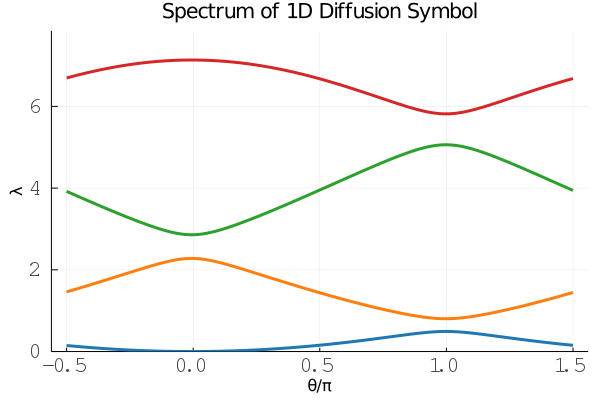
\includegraphics[height=3.9cm]{diffusionSymbol1D}
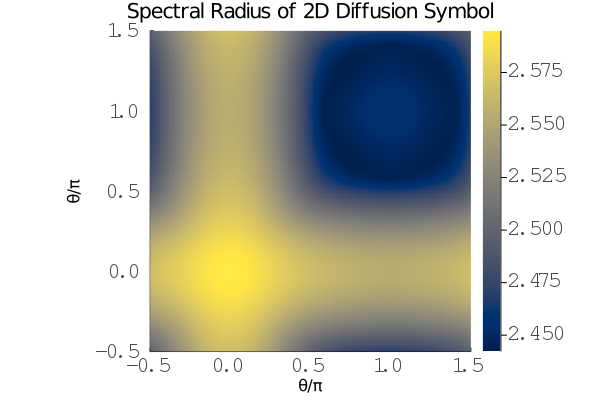
\includegraphics[height=3.9cm]{diffusionSymbol2D}
{\small Scalar Poisson problem on quartic elements}\\

~\\

Goal: decrease spectral radius with preconditioners

\end{center}
\end{frame}

%-------------------------------------------------------------------------------

\begin{frame}
\begin{center}
\frametitle{LFA of High-Order Smoothers}

Error propagation operator for smoothers given by

\vspace{-4mm}

\begin{equation}
\mathbf{S} = \mathbf{I} - \mathbf{M}^{-1} {\color{burgundy}A}
\end{equation}

~\\

with a symbol given by

\vspace{-4mm}

\begin{equation}
\tilde{\mathbf{S}} \left( \boldsymbol{\theta}, \omega \right) = \mathbf{I} - \tilde{\mathbf{M}}^{-1} \left( \boldsymbol{\theta}, \omega \right) \tilde{{\color{burgundy}A}} \left( \boldsymbol{\theta} \right)
\end{equation}

\end{center}
\end{frame}

%-------------------------------------------------------------------------------
\section{LFA of P-Multigrid Methods}
%-------------------------------------------------------------------------------

\begin{frame}
\begin{center}
\frametitle{Two-Grid Multigrid Error}

Multigrid methods target the low frequency error\\

\begin{equation}
\mathbf{E}_{\text{2MG}} = {\color{burgundy}\mathbf{S}}_f \left( \mathbf{I} - {\color{burgundy}\mathbf{P}}_{\text{ctof}} {\color{burgundy}\mathbf{A}}_c^{-1} {\color{burgundy}\mathbf{R}}_{\text{ftoc}} {\color{burgundy}\mathbf{A}}_f \right) {\color{burgundy}\mathbf{S}}_f
\end{equation}

\begin{itemize}

\item ${\color{burgundy}\mathbf{A}}_f$ - fine grid operator

\item ${\color{burgundy}\mathbf{A}}_c^{-1}$ - coarse grid solve (low frequency error)

\item ${\color{burgundy}\mathbf{S}}_f$ - fine grid smoother (high frequency error)

\item ${\color{burgundy}\mathbf{P}}_{\text{ctof}}$ - coarse to fine grid prolongation operator

\item ${\color{burgundy}\mathbf{R}}_{\text{ftoc}}$ - fine to coarse grid restriction operator

\end{itemize}

~\\

Grid transfer operators and coarse representation differentiate\\$h$-multigrid and $p$-multigrid

\end{center}
\end{frame}

%-------------------------------------------------------------------------------

\begin{frame}
\begin{center}
\frametitle{Two-Grid Multigrid Error}

The definition of the symbol follows naturally:\\

\begin{equation}
\tilde{\mathbf{E}}_{\text{2MG}} \left( \boldsymbol{\theta} \right) = \tilde{{\color{burgundy}\mathbf{S}}}_f \left( \boldsymbol{\theta}, \omega \right) \left( \mathbf{I} - \tilde{{\color{burgundy}\mathbf{P}}}_{\text{ctof}} \left( \boldsymbol{\theta} \right) \tilde{{\color{burgundy}\mathbf{A}}}_c^{-1} \left( \boldsymbol{\theta} \right) \tilde{{\color{burgundy}\mathbf{R}}}_{\text{ftoc}} \left( \boldsymbol{\theta} \right) \tilde{{\color{burgundy}\mathbf{A}}}_f \left( \boldsymbol{\theta} \right) \right) \tilde{{\color{burgundy}\mathbf{S}}}_f \left( \boldsymbol{\theta}, \omega \right)
\end{equation}

\begin{itemize}

\item $\tilde{{\color{burgundy}\mathbf{A}}}_f$ - fine grid symbol

\item $\tilde{{\color{burgundy}\mathbf{A}}}_c^{-1}$ - coarse grid symbol inverse (low frequency error)

\item $\tilde{{\color{burgundy}\mathbf{S}}}_f$ - fine grid smoother symbol (high frequency error)

\item $\tilde{{\color{burgundy}\mathbf{P}}}_{\text{ctof}}$ - coarse to fine grid prolongation symbol

\item $\tilde{{\color{burgundy}\mathbf{R}}}_{\text{ftoc}}$ - fine to coarse grid restriction symbol

\end{itemize}

\end{center}
\end{frame}

%-------------------------------------------------------------------------------

\begin{frame}
\begin{center}
\frametitle{{\textit P}-Multigrid Transfer Operators}

$p$-multigrid prolongation can be represented as an interpolation\\from the coarse to fine grid\\

\begin{columns}[onlytextwidth]
  \begin{column}{0.45\textwidth}
   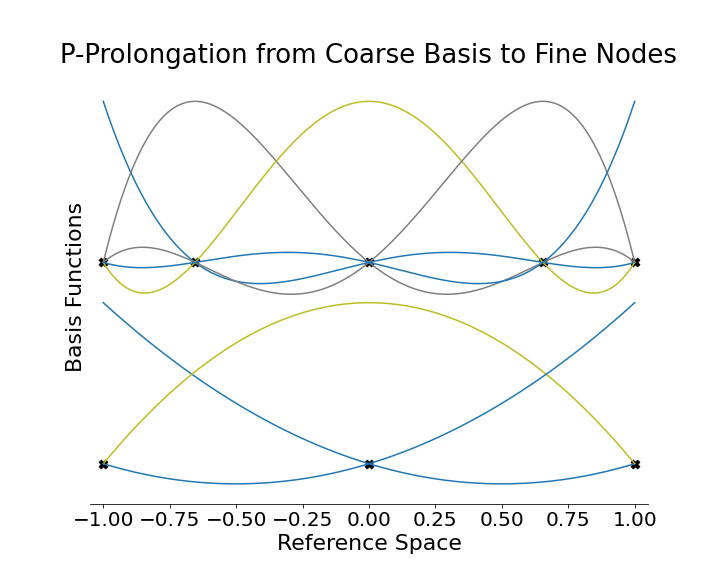
\includegraphics[width=1.0\textwidth]{pProlongation}
  \end{column}

  \begin{column}{0.45\textwidth}
  \begin{equation}
  \begin{gathered}
  {\color{burgundy}\mathbf{P}}_{\text{ctof}} = {\color{burgundy}\mathcal{P}}_f^T \mathcal{E}_f^T {\color{burgundy}\mathbf{P}}^e \mathcal{E}_c {\color{burgundy}\mathcal{P}}_c\\
  {\color{burgundy}\mathbf{P}}^e = {\color{blue(ncs)}\mathbf{I}} {\color{applegreen}\mathbf{D}}_{\text{scale}} {\color{blue(ncs)}\mathbf{B}}_{\text{ctof}}
  \end{gathered}
  \end{equation}

  $\color{applegreen}\mathbf{D}$ scales for node multiplicity
  \end{column}
\end{columns}

\end{center}
\end{frame}

%-------------------------------------------------------------------------------

\begin{frame}
\begin{center}
\frametitle{Example: {\textit P}-Multigrid}

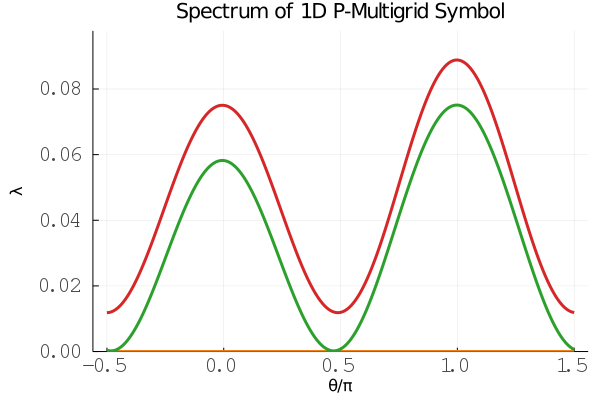
\includegraphics[height=3.9cm]{pmultigridSymbol1D}
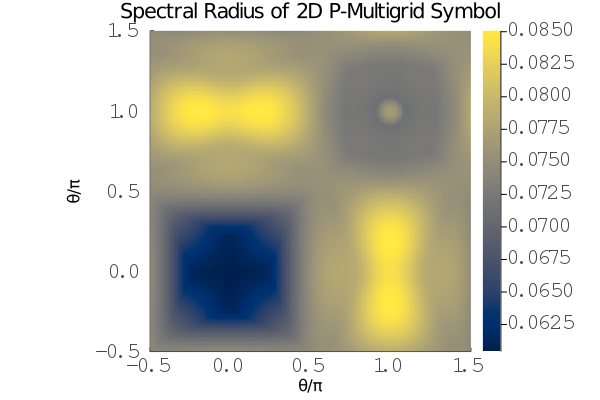
\includegraphics[height=3.9cm]{pmultigridSymbol2D}
{\small $p$-multigrid with third order Chebyshev on quartic to quadratic elements}\\

~\\

Significant reduction in spectral radius

\end{center}
\end{frame}

%-------------------------------------------------------------------------------

\begin{frame}
\begin{center}
\frametitle{Agressive Coarsening}

\begin{itemize}

\item High-order fine grid is most efficient representation\\

~\\

\item Linear coarse grid is easier to solve with traditional methods\\

~\\

\item Want to reduce number of intermediate grids\\

~\\

\item Typical smoothers do not respond well to agressive coarsening\\

\end{itemize}

\end{center}
\end{frame}

%-------------------------------------------------------------------------------

\begin{frame}
\begin{center}
\frametitle{Experiments: {\textit P}-Multigrid with Chebyshev}

\begin{table}[ht!]
\begin{center}
\begin{tabular}{l ccc ccc}
  \toprule
  $p_{\text{fine}}$ to $p_{\text{coarse}}$  &  \multicolumn{3}{c}{$k = 3$}  &  \multicolumn{3}{c}{$k = 4$}  \\
                      &  LFA    &  libCEED  &  its  &  LFA   &  libCEED  &  its  \\
  \toprule
  $p = 2$ to $p = 1$  &  0.076  &  0.058    &  9    &  0.041 &  0.033    &  7    \\
  \midrule
  $p = 4$ to $p = 2$  &  0.111  &  0.097    &  10   &  0.062  &  0.050   &  8    \\
  $p = 4$ to $p = 1$  &  0.416  &  0.398    &  25   &  0.295  &  0.276   &  18   \\
  \midrule
  $p = 8$ to $p = 4$  &  0.197  &  0.195    &  15   &  0.121  &  0.110   &  11   \\
  $p = 8$ to $p = 2$  &  0.611  &  0.603    &  46   &  0.506  &  0.469   &  31   \\
  $p = 8$ to $p = 1$  &  0.871  &  0.861    &  154  &  0.827  &  0.814   &  112  \\
  \bottomrule
\end{tabular}
\end{center}
\label{table:two_grid_3d_chebyshev}
\end{table}
{\small LFA and experimental two-grid convergence factors with\\Chebyshev smoothing for 3D Laplacian}\\

~\\

3D manufactured solution on the domain $\left[ -3, 3 \right]^3$ with Dirichlet boundaries:

\begin{equation}
f \left( x, y, z \right) = x y z \sin \left( \pi x \right) \sin \left( \pi \left( 1.23 + 0.5 y \right) \right) \sin \left( \pi \left( 2.34 + 0.25 z \right) \right)
\end{equation}

\end{center}
\end{frame}

%-------------------------------------------------------------------------------
\section{LFA of BDDC}
%-------------------------------------------------------------------------------

\begin{frame}
\begin{center}
\frametitle{BDDC Overview}

\includegraphics[height=4.5cm]{HighOrderBDDCMeshInterface}\\
{\small High-order single element subdomains}\\

~\\

BDDC - non-overlapping domain decomposition method by Dohrmann\\

\end{center}
\end{frame}

%-------------------------------------------------------------------------------

\begin{frame}
\begin{center}
\frametitle{Broken Subdomains}

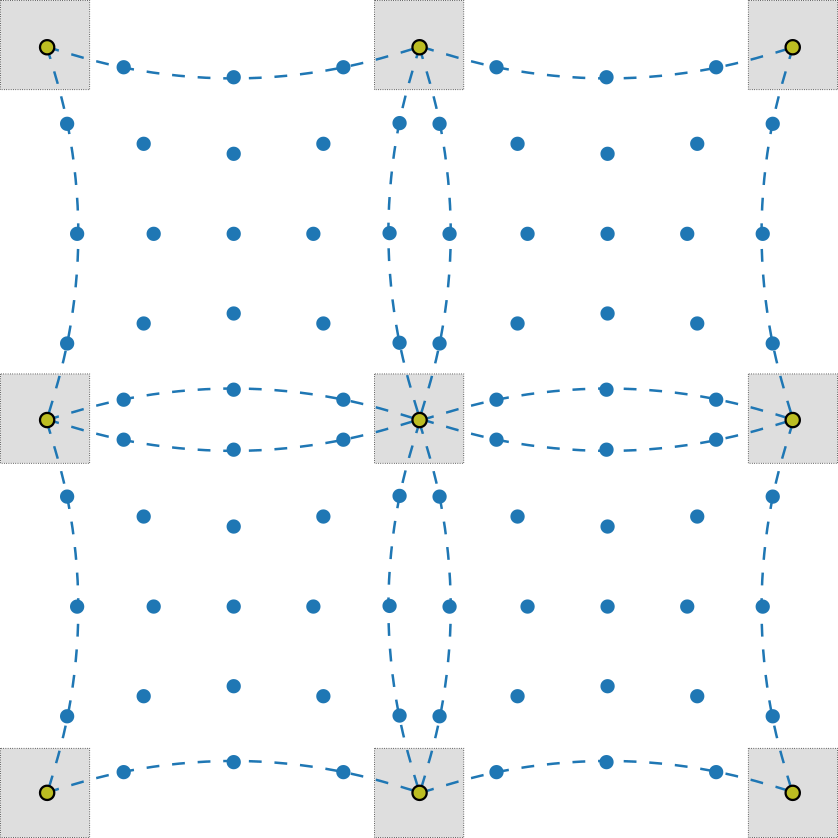
\includegraphics[height=4.5cm]{HighOrderBDDCMeshPrimal}
\hspace{10mm}
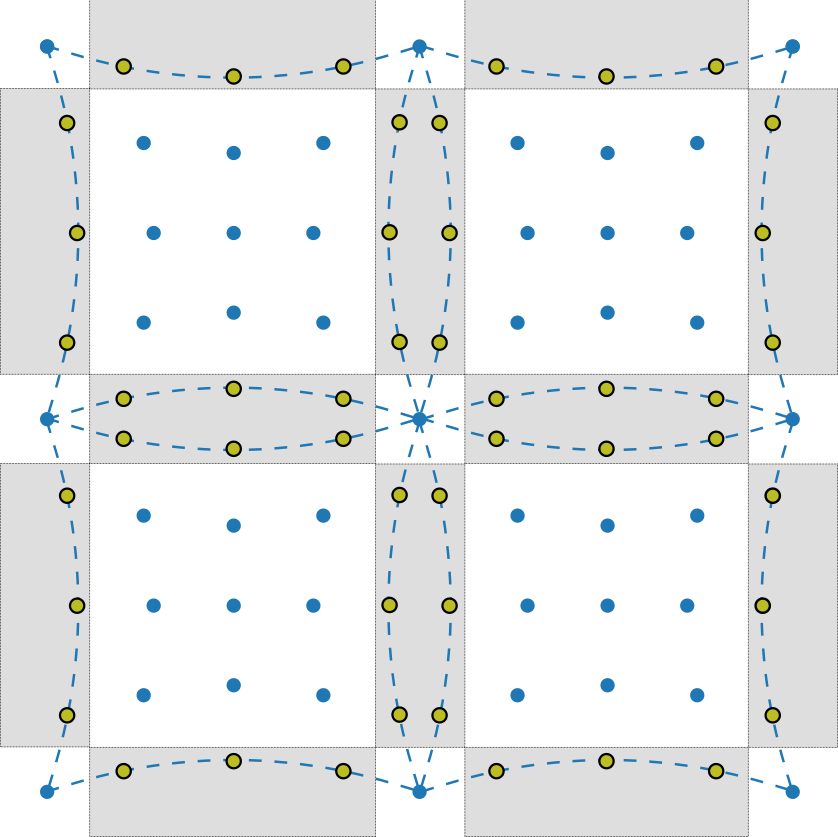
\includegraphics[height=4.5cm]{HighOrderBDDCMeshInterfaceBroken}\\
{\small Non-overlapping domain decomposition of high-order mesh}\\

~\\

Global problem only "partially subassembled" on primal ($\Pi$) vertices\\

~\\

Remaining interface nodes replicated across broken interface

\end{center}
\end{frame}

%-------------------------------------------------------------------------------

\begin{frame}
\begin{center}
\frametitle{Subassembled Problem}

\begin{equation}
\hat{\color{burgundy}\mathbf{A}}^{-1} = \sum_{e = 1}^N \mathbf{R}^{e, T}_i \hat{\color{burgundy}\mathbf{A}}^{e, -1} \mathbf{R}^e_i, \hspace{10mm}
\hat{\color{burgundy}\mathbf{A}}^e =
\left[ \begin{array}{c c}
{\color{burgundy}\mathbf{A}}_{\text{r}, \text{r}}^e  &  \hat{\color{burgundy}\mathbf{A}}_{\Pi, \text{r}}^{e, T}  \\
\hat{\color{burgundy}\mathbf{A}}_{\Pi, \text{r}}^e   &  \hat{\color{burgundy}\mathbf{A}}_{\Pi, \Pi}^e            \\
\end{array} \right]
\end{equation}

Partially subassembled problem is easier to invert\\

~\\

Injection operator $\mathbf{R}_i$ maps from global space to broken space\\and provides different BDDC variants

\end{center}
\end{frame}

%-------------------------------------------------------------------------------

\begin{frame}
\begin{center}
\frametitle{Injection Operators}

\begin{columns}[onlytextwidth]
  \begin{column}{0.49\textwidth}
  \begin{center}

  \begin{equation}
  \mathbf{R}_1 = \diag \left( \left[ \frac{1}{\lvert \mathcal{N} \left( x_i \right) \rvert} \right] \right)
  \end{equation}

  where $\lvert \mathcal{N} \left( x_i \right) \rvert$ is node multiplicity across broken spaces\\
  \end{center}
  \end{column}

  \begin{column}{0.45\textwidth}
  \begin{center}
  \begin{equation}
  \begin{gathered}
  \mathbf{R}_2 = \mathbf{R}_1 - \mathbf{J}^T \boldsymbol{\mathcal{H}}^T\\
  \boldsymbol{\mathcal{H}}^e = - {\color{burgundy}\mathbf{A}}_{\text{I}, \text{I}}^{e, -1} {\color{burgundy}\mathbf{A}}_{\Gamma, \text{I}}^{e, T}
  \end{gathered}
  \end{equation}

  where $\boldsymbol{\mathcal{H}}$ is a harmonic extension,\\$\mathbf{J}$ a map over the interfaces
  \end{center}
  \end{column}
\end{columns}

~\\

~\\

Lumped BDDC with $\mathbf{R}_1$ cheaper to setup but poorer conditioning\\

~\\

Dirichlet BDDC with $\mathbf{R}_2$ equivalent to Dirichlet FETI-DP

\end{center}
\end{frame}

%-------------------------------------------------------------------------------

\begin{frame}
\begin{center}
\frametitle{Subassembled Inverse}

\begin{equation}
\hat{\color{burgundy}\mathbf{A}}^e =
\left[ \begin{array}{c c}
{\color{burgundy}\mathbf{A}}_{\text{r}, \text{r}}^e  &  \hat{\color{burgundy}\mathbf{A}}_{\Pi, \text{r}}^{e, T}  \\
\hat{\color{burgundy}\mathbf{A}}_{\Pi, \text{r}}^e   &  \hat{\color{burgundy}\mathbf{A}}_{\Pi, \Pi}^e            \\
\end{array} \right] \hspace{10mm}
\hat{\mathbf{S}}_\Pi = {\color{burgundy}\mathbf{A}}_{\Pi, \Pi} - \hat{\color{burgundy}\mathbf{A}}_{\Pi, r} {\color{burgundy}\mathbf{A}}_{r, r}^{-1} \hat{\color{burgundy}\mathbf{A}}_{\Pi, r}^T
\label{eq:subassembledschur}
\end{equation}

\begin{itemize}

\item Subassembled problem inverted with Schur complement\\

~\\

\item Coarse grid problem $\hat{\mathbf{S}}_\Pi$ is easier to solve with traditional methods\\

~\\

\item Dense high-order element interior inverse ${\color{burgundy}\mathbf{A}}_{r, r}^{-1}$ can be expensive\\

~\\

\item Fast diagonalization can provide effiecient approximate solver\\

\end{itemize}

\end{center}
\end{frame}

%-------------------------------------------------------------------------------

\begin{frame}
\begin{center}
\frametitle{Fast Diagonalization}

For separable problems of the form

\vspace{-4mm}

\begin{equation}
\mathbf{A} = a \mathbf{M} + b \mathbf{K}
\end{equation}

Fast Diagonalization provides fast approximate solver

\vspace{-4mm}

\begin{equation}
\mathbf{A}^{-1} = \mathbf{S}^T \left( a \mathbf{I} + b \boldsymbol{\Lambda} \right)^{-1} \mathbf{S}
\label{eq:fdminverse}
\end{equation}

where

\vspace{-4mm}

\begin{equation}
\mathbf{S} \mathbf{M} \mathbf{S}^T = \mathbf{I}, \hspace{2mm} \mathbf{S} \mathbf{K} \mathbf{S}^T = \boldsymbol{\Lambda}
\end{equation}

\end{center}
\end{frame}

%-------------------------------------------------------------------------------

\begin{frame}
\begin{center}
\frametitle{Fast Diagonalization}

\begin{itemize}

\item Tensor product bases have tensor product diagonalizations\\

~\\

\item Convergence impact of approximate solver formulations is\\ongoing research\\

~\\

\item Cheaper to compute Fast Diagonalization solver than invert\\assembled subdomain matrices\\

~\\

\item Reusing diagonalization for injection subdomain operator inverse mitigates expensive setup cost of Dirichlet BDDC\\

\end{itemize}

\end{center}
\end{frame}

%-------------------------------------------------------------------------------

\begin{frame}
\begin{center}
\frametitle{LFA of BDDC}

\begin{equation}
\tilde{\hat{\color{burgundy} \mathbf{A}}}\color{black}^{-1} =
\left[ \begin{array}{c c}
\mathbf{I}  &  -\tilde{\color{burgundy}\mathbf{A}}_{\text{r}, \text{r}}^{-1} \tilde{\hat{\color{burgundy}\mathbf{A}}}\color{black}_{\Pi, \text{r}}^T  \\
\mathbf{0}  &  \mathbf{I}                                                                                                                             \\
\end{array} \right]
\left[ \begin{array}{c c}
\tilde{\color{burgundy}\mathbf{A}}_{\text{r}, \text{r}}^{-1}  &  \mathbf{0}                                        \\
\mathbf{0}                                                    &  \tilde{\hat{\mathbf{S}}}\color{black}_{\Pi}^{-1}  \\
\end{array} \right]
\left[ \begin{array}{c c}
\mathbf{I}                                                                                                                           &  \mathbf{0}  \\
-\tilde{\color{burgundy}\mathbf{A}}_{\Pi, \text{r}} \tilde{\hat{\color{burgundy}\mathbf{A}}}\color{black}_{\text{r}, \text{r}}^{-1}  &  \mathbf{I}  \\
\end{array} \right]
\end{equation}

\begin{equation}
\begin{gathered}
\tilde{\color{burgundy}\mathbf{A}}_{\text{r}, \text{r}}^{-1} \left( \boldsymbol{\theta} \right) = {\color{burgundy}\mathbf{A}}_{\text{r}, \text{r}}^{-1} \odot \left[ e^{\imath \left( \mathbf{x}_j - \mathbf{x}_i \right) \cdot \boldsymbol{\theta} / \mathbf{h}} \right],
\hspace{5mm}
\tilde{\hat{\color{burgundy}\mathbf{A}}}\color{black}_{\text{r}, \Pi} \left( \boldsymbol{\theta} \right) = \left( \hat{\color{burgundy}\mathbf{A}}_{\text{r}, \Pi} \odot \left[ e^{\imath \left( \mathbf{x}_j - \mathbf{x}_i \right) \cdot \boldsymbol{\theta} / \mathbf{h}} \right] \right) \mathbf{Q}_{\Pi},\\
\tilde{\hat{\mathbf{S}}}_{\Pi}^{-1} \left( \boldsymbol{\theta} \right) = \left( \mathbf{Q}_{\Pi}^T \left( \hat{\mathbf{S}}_{\Pi} \odot \left[ e^{\imath \left( \mathbf{x}_j - \mathbf{x}_i \right) \cdot \boldsymbol{\theta} / \mathbf{h}} \right] \right) \mathbf{Q}_{\Pi} \right)^{-1}
\end{gathered}
\end{equation}

Only primal modes are localized for subassembled operator symbol\\

~\\

Symbols of injection operators are relatively straightforward\\

\end{center}
\end{frame}

%-------------------------------------------------------------------------------

\begin{frame}
\begin{center}
\frametitle{Low-Order Validation}

\begin{table}[ht!]
\begin{center}
\begin{tabular}{l ccc ccc}
  \toprule
  $m$  &  \multicolumn{3}{c}{Lumped BDDC}  &  \multicolumn{3}{c}{Dirichlet BDDC}  \\
                      &  $\lambda_{\min}$  &  $\lambda_{\max}$  &  $\kappa$ & $\lambda_{\min}$  &  $\lambda_{\max}$ & $\kappa$  \\
  \toprule
  $m = 4$   &  1.000  &   4.444  &   4.444  &  1.000  &  2.351  &  2.351  \\
  $m = 8$   &  1.000  &  12.269  &  12.269  &  1.000  &  3.196  &  3.196  \\
  $m = 16$  &  1.000  &  31.179  &  31.179  &  1.000  &  4.188  &  4.188  \\
  $m = 32$  &  1.000  &  75.761  &  75.761  &  1.000  &  5.335  &  5.335  \\
  \bottomrule
\end{tabular}
\end{center}
\label{table:macro_element_bddc}
\end{table}
{\small Condition numbers and maximal eigenvalues\\for low-order macro-elements}\\

~\\

Exactly reproduces original work on LFA of low-order subdomains (Brown and He)

\end{center}
\end{frame}

%-------------------------------------------------------------------------------

\begin{frame}
\begin{center}
\frametitle{High-Order Experiments}

\begin{table}[ht!]
\begin{center}
\begin{tabular}{l ccc ccc}
  \toprule
  $p$  &  \multicolumn{3}{c}{Lumped BDDC}  &  \multicolumn{3}{c}{Dirichlet BDDC}  \\
                      &  $\lambda_{\min}$  &  $\lambda_{\max}$  &  $\kappa$ & $\lambda_{\min}$  &  $\lambda_{\max}$ & $\kappa$  \\
  \toprule
  $p = 2$   &  1.000  &    2.800  &    2.800  &  1.000  &  2.042  &  2.042  \\
  $p = 4$   &  1.000  &   12.948  &   12.948  &  1.000  &  3.242  &  3.242  \\
  $p = 8$   &  1.000  &   59.563  &   59.563  &  1.000  &  5.197  &  5.197  \\
  $p = 16$  &  1.000  &  289.678  &  289.678  &  1.000  &  7.761  &  7.761  \\
  \bottomrule
\end{tabular}
\end{center}
\label{table:high_order_element_bddc}
\end{table}
{\small Condition numbers and maximal eigenvalues\\for single high-order element subdomains}\\

~\\

Single high-order element subdomains less well conditioned

\end{center}
\end{frame}

%-------------------------------------------------------------------------------

\begin{frame}
\begin{center}
\frametitle{Low vs High-Order BDDC}

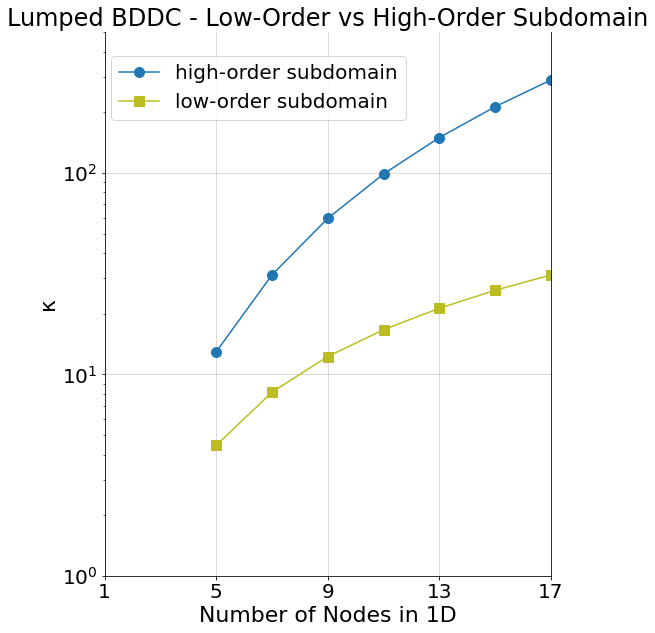
\includegraphics[height=5.3cm]{lowVsHighLumped_tall}
\hspace{0.3cm}
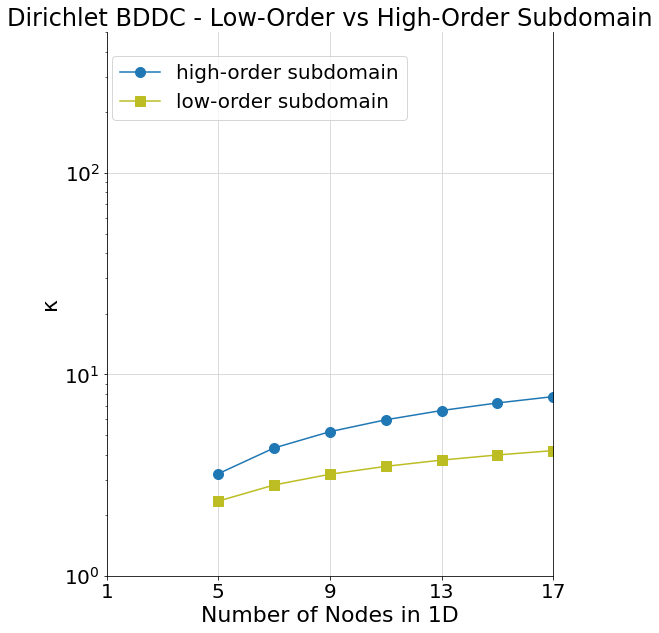
\includegraphics[height=5.3cm]{lowVsHighDirichlet_tall}
{\small Low-order and high-order subdomain condition number}\\

~\\

Dirichlet BDDC important for single high-order element subdomains

\end{center}
\end{frame}

%-------------------------------------------------------------------------------

\begin{frame}
\begin{center}
\frametitle{BDDC Smoother for $P$-Multigrid}

\begin{columns}[onlytextwidth]
  \begin{column}{0.49\textwidth}
  \begin{center}
  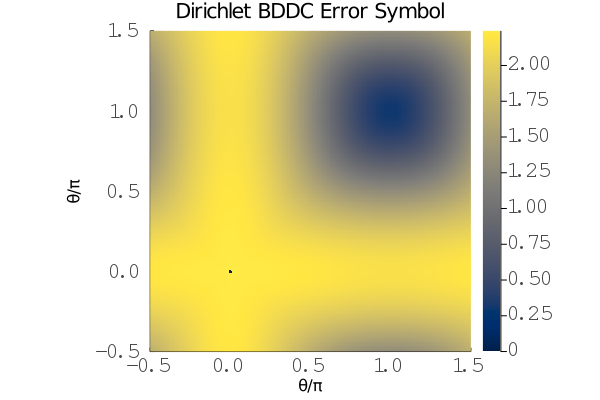
\includegraphics[width=1.0\textwidth]{DirichletBDDCHighOrderNoRelaxation}
  {\small Symbol of error operator for Dirichlet BDDC of 2D Laplacian for $p = 4$}
  \end{center}
  \end{column}

  \begin{column}{0.45\textwidth}
  \begin{center}
  Dirichlet BDDC smoother still has large spectral radius, so we introduce relaxation parameter\\

  ~\\

  \begin{equation}
  \tilde{\mathbf{E}} \left( \boldsymbol{\theta}, \omega \right) = \mathbf{I} - \omega \tilde{\mathbf{M}}_2^{-1} \tilde{{\color{burgundy}A}} \left( \boldsymbol{\theta} \right)
  \end{equation}
  \end{center}
  \end{column}
\end{columns}

\end{center}
\end{frame}

%-------------------------------------------------------------------------------

\begin{frame}
\begin{center}
\frametitle{BDDC Smoother for $P$-Multigrid}

\begin{table}[ht!]
\begin{center}
\begin{tabular}{l ccc cc}
  \toprule
  $p_{\text{fine}}$ to $p_{\text{coarse}}$  & \multicolumn{3}{c}{Dirichlet BDDC} & \multicolumn{2}{c}{Chebyshev}  \\
   &  $\rho$ & $\omega_{\text{opt}}$  & its  & $\rho$  &  its  \\
  \toprule
  $p = 2$ to $p = 1$   &  0.121  &  0.66  &  11  &  0.075  &  9    \\
  \midrule
  $p = 4$ to $p = 2$   &  0.272  &  0.48  &  18  &  0.085  &  10   \\
  $p = 4$ to $p = 1$   &  0.281  &  0.47  &  19  &  0.219  &  16   \\
  \midrule
  $p = 8$ to $p = 4$   &  0.409  &  0.38  &  26  &  0.110  &  11   \\
  $p = 8$ to $p = 1$   &  0.462  &  0.32  &  30  &  0.795  &  101  \\
  \midrule
  $p = 16$ to $p = 8$  &  0.504  &  0.32  &  34  &  0.435  &  28   \\
  $p = 16$ to $p = 1$  &  0.597  &  0.23  &  45  &  0.959  &  551  \\
  \bottomrule
\end{tabular}
\end{center}
\label{table:two_grid_bddc_smoother_vs_cubic_chebyshev}
\end{table}
{\small Two-grid convergence factor for $p$-multigrid with BDDC\\vs cubic Chebyshev smoothing for 2D Laplacian}\\

~\\

Weighted Dirichlet BDDC smoother better supports rapid coarsening\\

\end{center}
\end{frame}

%-------------------------------------------------------------------------------

\begin{frame}
\begin{center}
\frametitle{BDDC Smoother for $P$-Multigrid}

\begin{table}[ht!]
\begin{center}
\begin{tabular}{l ccc cc}
  \toprule
  $p_{\text{fine}}$ to $p_{\text{coarse}}$  & \multicolumn{3}{c}{Dirichlet BDDC} & \multicolumn{2}{c}{Chebyshev}  \\
   &  $\rho$ & $\omega_{\text{opt}}$  & its  & $\rho$  &  its  \\
  \toprule
  $p = 2$ to $p = 1$   &  0.121  &  0.66  &  11  &  0.252  &  17   \\
  \midrule
  $p = 4$ to $p = 2$   &  0.272  &  0.48  &  18  &  0.281  &  19   \\
  $p = 4$ to $p = 1$   &  0.281  &  0.47  &  19  &  0.424  &  27   \\
  \midrule
  $p = 8$ to $p = 4$   &  0.409  &  0.38  &  26  &  0.278  &  18   \\
  $p = 8$ to $p = 1$   &  0.462  &  0.32  &  30  &  0.873  &  170  \\
  \midrule
  $p = 16$ to $p = 8$  &  0.504  &  0.32  &  34  &  0.613  &  48   \\
  $p = 16$ to $p = 1$  &  0.597  &  0.23  &  45  &  0.975  &  910  \\
  \bottomrule
\end{tabular}
\end{center}
\label{table:two_grid_bddc_smoother_vs_quadratic_chebyshev}
\end{table}
{\small Two-grid convergence factor for $p$-multigrid with BDDC\\vs quadratic Chebyshev smoothing for 2D Laplacian}\\

~\\

Weighted Dirichlet BDDC smoother better supports rapid coarsening\\

\end{center}
\end{frame}

%-------------------------------------------------------------------------------
\section{Summary}
%-------------------------------------------------------------------------------

\begin{frame}
\begin{center}
\frametitle{Summary}

\begin{itemize}

\item High-order matrix-free representations of PDEs are better suited to modern hardware than sparse matrices\\

~\\

\item High-order matrix-free representations require preconditioned\\iterative solvers\\

~\\

\item Local Fourier Analysis (LFA) provides sharp convergence estimates\\for these preconditioners\\

~\\

\item We investigated LFA of Balancing Domain Decomposition by Constraints (BDDC) for high-order element subdomains\\

~\\

\item Finally, we investigated LFA of $p$-multigrid with a BDDC smoother

\end{itemize}

\end{center}
\end{frame}

%-------------------------------------------------------------------------------

\begin{frame}[noframenumbering]
\titlepage % Print the title page
\end{frame}

%-------------------------------------------------------------------------------

\end{document}

%-------------------------------------------------------------------------------
